\documentclass[11pt]{article}
\usepackage[margin=1in]{geometry}
\usepackage{amsmath,amssymb,amsthm}
\usepackage{graphicx}
\usepackage{hyperref}
\usepackage{xcolor}

\newtheorem{theorem}{Theorem}
\newtheorem{lemma}{Lemma}
\newtheorem{remark}{Remark}

\newcommand{\R}{\mathbb{R}}
\newcommand{\eps}{\varepsilon}
\newcommand{\ot}{\otimes}
\newcommand{\abs}[1]{\left|#1\right|}
\newcommand{\norm}[1]{\left\|#1\right\|}

\title{A computer-certified \(8/7\) universal projective/injective gap}
\author{Run \texttt{fa\_banach\_001}, lane 15}
\date{2026-06-16}

\begin{document}
\maketitle

\section*{Status}

This packet records a claimed partial result for the open problem of Aubrun,
Lami, Palazuelos, Szarek, and Winter \cite{ALPSW}: whether
\(\rho(X,Y)\geq \sqrt2\) for all real Banach spaces \(X,Y\) of dimension at
least \(2\).  The result below does not reach \(\sqrt2\), but it improves the
paper's universal lower bound \(19/18\) to \(8/7\).  This is exactly the
computer-assisted improvement suggested, but not presented, in the remark after
the proof of Theorem 2 of \cite{ALPSW}.

\begin{figure}[h]
\centering

\includegraphics[width=0.92\linewidth]{figures/open_problem_crop.png}
\caption{Problem 3 in \cite{ALPSW}, asking whether the universal gap is
\(\sqrt2\).}
\end{figure}

\begin{figure}[h]
\centering
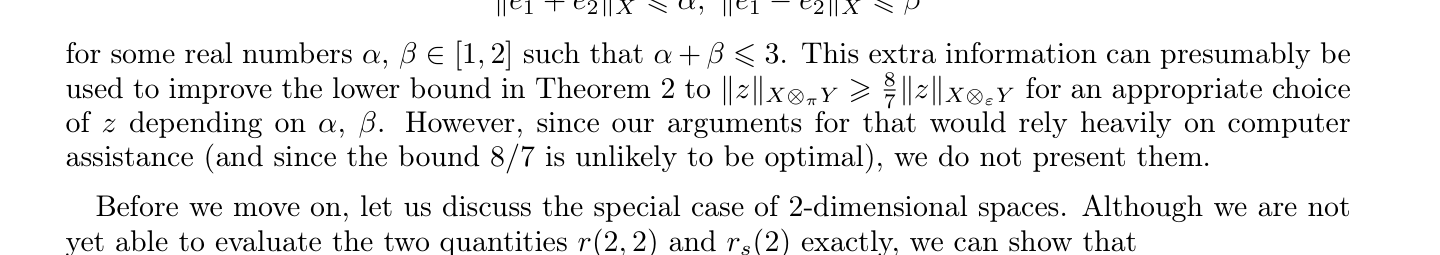
\includegraphics[width=0.92\linewidth]{figures/eight_over_seven_remark_crop.png}
\caption{The source-paper remark suggesting the \(8/7\) improvement from the
refined Auerbach data.}
\end{figure}

\section*{Definitions}

For Banach spaces \(X,Y\), let
\[
\rho(X,Y)=
\sup_{0\neq z\in X\ot Y}
\frac{\norm{z}_{X\ot_\pi Y}}{\norm{z}_{X\ot_\eps Y}} .
\]
Equivalently, \(\rho(X,Y)\) is the best domination constant of the injective
norm by the projective norm on \(X\ot Y\).  The source paper defines
\[
r(n,m)=\inf_{\dim X=n,\ \dim Y=m}\rho(X,Y).
\]

\section*{Proof Intuition}

The proof of the \(19/18\) theorem in \cite{ALPSW} uses a two-dimensional
Auerbach argument and then tests a CHSH-type functional against a carefully
chosen \(2\times2\) tensor.  The source paper deliberately discards half of the
geometric information produced by the Auerbach step: besides one diagonal
bound, the proof actually gives two bounds
\[
\norm{e_1+e_2}\leq \alpha,\qquad \norm{e_1-e_2}\leq \beta,\qquad
\alpha+\beta\leq 3 .
\]
Keeping both bounds changes the coordinate body from a hexagon with one strip
constraint to a clipped square with two strip constraints.  The tensor can then
be chosen adaptively from a small linear program.  The worst case occurs at the
balanced octagon \(\alpha=\beta=3/2\), where the certificate is simply
\((4/7)\) times the usual CHSH tensor.  Away from the balanced case there is
extra room, and the exact verifier checks the resulting finite family of
polynomial inequalities.

\section*{Main Result}

\begin{theorem}
\label{thm:eight-sevenths}
Let \(X\) and \(Y\) be real Banach spaces with
\(\dim X,\dim Y\geq 2\).  Then
\[
\rho(X,Y)\geq \frac87 .
\]
Consequently, \(r(n,m)\geq 8/7\) for all \(n,m\geq 2\).
\end{theorem}

\begin{proof}
We use the refined form of Lemma 15 from \cite{ALPSW}.  Applied to \(X\), it
gives vectors \(e_1,e_2\in X\) and functionals
\(e_1^*,e_2^*\in X^*\) such that
\[
\norm{e_i}=\norm{e_i^*}=1,\qquad e_j^*(e_i)=\delta_{ij},
\]
and, for some \(\alpha,\beta\in[1,2]\),
\[
\norm{e_1+e_2}\leq \alpha,\qquad
\norm{e_1-e_2}\leq \beta,\qquad \alpha+\beta\leq 3.
\]
Apply the same construction in \(Y\), obtaining \(f_1,f_2\), \(f_1^*,f_2^*\)
and parameters \(\gamma,\delta\in[1,2]\) with \(\gamma+\delta\leq3\).

If necessary, enlarge the parameters while keeping them in \([1,2]\) until
\(\alpha+\beta=3\) and \(\gamma+\delta=3\).  This only enlarges the coordinate
sets used below and therefore makes the injective-norm estimate harder.  Thus
it suffices to prove the boundary case
\[
\alpha=1+m,\quad \beta=2-m,\quad
\gamma=1+r,\quad \delta=2-r
\]
with \(m,r\in[0,1]\).  Define
\[
H_m=\{(s,t)\in\R^2:\ |s|\leq1,\ |t|\leq1,\ |s+t|\leq1+m,\ |s-t|\leq2-m\}.
\]
For every \(\phi\in B_{X^*}\), the coordinate pair
\((\phi(e_1),\phi(e_2))\) lies in \(H_m\), and similarly the \(Y\)-coordinates
lie in \(H_r\).

The following certified finite-dimensional lemma is the only computer-assisted
part of the proof.

\begin{lemma}[certified two-parameter CHSH certificate]
\label{lem:certificate}
For every \(m,r\in[0,1]\) there exists a real \(2\times2\) matrix
\[
A(m,r)=\begin{pmatrix}a_{11}&a_{12}\\a_{21}&a_{22}\end{pmatrix}
\]
such that
\[
\abs{x^\mathsf{T}A(m,r)y}\leq 1
\quad\forall x\in H_m,\ \forall y\in H_r,
\]
and
\[
a_{11}+a_{12}+a_{21}-a_{22}\geq\frac{16}{7}.
\]
\end{lemma}

Assuming Lemma \ref{lem:certificate}, set
\[
z=\sum_{i,j=1}^2 a_{ij}\, e_i\ot f_j\in X\ot Y .
\]
The first assertion of the lemma gives
\[
\norm{z}_{X\ot_\eps Y}\leq1.
\]
Now consider the CHSH functional
\[
w^*=e_1^*\ot f_1^*+e_1^*\ot f_2^*
    +e_2^*\ot f_1^*-e_2^*\ot f_2^* .
\]
Since \(e_i^*\) and \(f_j^*\) have norm \(1\), the usual CHSH inequality gives
\[
\norm{w^*}_{X^*\ot_\eps Y^*}\leq2.
\]
Therefore, by duality,
\[
\norm{z}_{X\ot_\pi Y}
\geq \frac{\abs{w^*(z)}}{\norm{w^*}_{X^*\ot_\eps Y^*}}
\geq \frac{(16/7)}{2}=\frac87 .
\]
Since \(\norm{z}_{X\ot_\eps Y}\leq1\), this proves
\(\rho(X,Y)\geq8/7\).
\end{proof}

\section*{Proof of the Certified Lemma}

We give the exact finite certificate and point to the verifier implementing the
arithmetic.  On the boundary, the vertices of \(H_m\) are
\[
\begin{aligned}
&(1,m),\ (1,m-1),\ (-1,-m),\ (-1,1-m),\\
&(m,1),\ (m-1,1),\ (-m,-1),\ (1-m,-1),
\end{aligned}
\]
with the analogous list for \(H_r\).  Let \(A=A(m,r)\) be the unique solution
of the four linear equations
\[
\begin{aligned}
(1,m)^\mathsf{T}A(1,r)&=1,\\
(1,m-1)^\mathsf{T}A(r,1)&=1,\\
(m,1)^\mathsf{T}A(1,r-1)&=1,\\
(m-1,1)^\mathsf{T}A(r-1,1)&=-1.
\end{aligned}
\]
The entries of \(A\) are rational functions of \(m,r\).  The denominator is
strictly positive on the square \([0,1]^2\).  Because \(H_m\) and \(H_r\) are
polytopes and the form \(x^\mathsf{T}Ay\) is affine in each variable, it is
enough to check the \(8\cdot8\) vertex pairs.  Thus Lemma
\ref{lem:certificate} reduces to the following exact inequalities on
\([0,1]^2\):
\[
D(m,r)>0,
\]
\[
(1\pm v_i(m)^\mathsf{T}A(m,r)v_j(r))D(m,r)\geq0
\quad(0\leq i,j<8),
\]
and
\[
\left(a_{11}+a_{12}+a_{21}-a_{22}-\frac{16}{7}\right)D(m,r)\geq0.
\]

The verifier
\[
\texttt{code/verify\_8over7\_certificate.py}
\]
symbolically constructs these \(130\) polynomials and proves their
nonnegativity using exact rational Bernstein coefficients with recursive
subdivision.  The run included in this packet reports:
\[
\texttt{checks=130,\ failures=0,\ max\_depth\_used=2.}
\]

For orientation, at the balanced point \(m=r=1/2\) the certificate is
\[
A=\frac47
\begin{pmatrix}
1&1\\
1&-1
\end{pmatrix},
\]
and the inequality is tight for this certificate:
\[
a_{11}+a_{12}+a_{21}-a_{22}=\frac{16}{7}.
\]

\section*{Analytic Audit of the Certificate}

The helper
\[
\texttt{code/analyze\_certificate\_symmetry.py}
\]
gives a more reviewable view of the same exact certificate.  Under the
symmetries \(m\leftrightarrow1-m\), \(r\leftrightarrow1-r\), and
\(m\leftrightarrow r\), the \(130\) polynomial checks collapse to \(10\)
representative classes.  Each representative is then checked on the four
quadrants of the centered square by exact Bernstein coefficients.

The most important representative, the objective inequality, has a simple
hand proof.  Put \(x=2m-1\), \(y=2r-1\), \(X=x^2\), and \(Y=y^2\).  After
clearing the positive scalar factor, the numerator of the objective class is
\[
X^2Y^2-10X^2Y+9X^2-10XY^2+51XY+15X+9Y^2+15Y.
\]
On \(0\leq X,Y\leq1\) this equals
\[
X^2(1-Y)(9-Y)+X(-10Y^2+51Y+15)+9Y^2+15Y,
\]
which is nonnegative.  Thus the tight part of the certificate is already
elementary; the remaining nontrivial vertex classes are the part still best
audited through the exact Bernstein atlas.

\section*{Verification Notes}

The proof uses only:
\begin{itemize}
\item Lemma 15 and its stated refinement from \cite{ALPSW};
\item the elementary CHSH bound for four scalar variables in \([-1,1]\);
\item the exact rational verifier included with this packet.
\end{itemize}
The verifier does not call a numerical optimizer.  The earlier LP searches were
used only to discover the four defining equations for \(A(m,r)\).

\section*{Limitations and Novelty Check}

This does not solve Problem 3 of \cite{ALPSW}: the conjectural sharp lower
bound \(\sqrt2\) remains open.  The result is a universal constant improvement
\[
19/18\quad\longrightarrow\quad 8/7.
\]

Local run indexes were checked for arXiv id \(\texttt{1809.10616}\), the title,
``projective/injective ratio'', ``XOR games'', ``sqrt(2)'', and ``8/7''; no
existing promoted packet was found.  A bounded web search for exact phrases
around \(\rho(X,Y)\), ``projective-injective ratio'', ``sqrt(2)'', and ``8/7''
found the source paper but no obvious later paper presenting this certificate
or resolving the \(\sqrt2\) problem.  Novelty confidence is therefore
moderate-high, subject to expert literature review.

\section*{Human Review Recommendation}

Recommended review focus:
\begin{enumerate}
\item check that the refined Auerbach data from Lemma 15 of \cite{ALPSW}
indeed applies independently to \(X\) and \(Y\) in the form used here;
\item audit the exact verifier, especially the four equations defining
\(A(m,r)\), the vertex list for \(H_m\), and the Bernstein nonnegativity
routine;
\item confirm that enlarging to the boundary \(\alpha+\beta=\gamma+\delta=3\)
is legitimate for the injective-norm upper bound.
\end{enumerate}
If these checks pass, this packet should be treated as a likely valid partial
result toward Problem 3.

\begin{thebibliography}{9}
\bibitem{ALPSW}
G. Aubrun, L. Lami, C. Palazuelos, S. J. Szarek, and A. Winter,
\emph{Universal gaps for XOR games from estimates on tensor norm ratios},
arXiv:1809.10616.
\end{thebibliography}

\end{document}
